\documentclass{assignmeownt}

\usepackage{graphicx}
% \usepackage[table]{xcolor}
\usepackage{colortbl}
\usepackage{booktabs}
\graphicspath{ {./images/} }

\coursenumber{MTL782}
\coursetitle{Data Mining}
\doctitle{Assignment 2}
\docauthor{Saket Kandoi 2021MT60265 \\ Navneet Raj 2021MT10240 \\ Aditya Thomas 2021MT60944}

\definecolor{lightblu}{RGB}{217, 235, 255}
\definecolor{darkblue}{RGB}{0, 51, 102}

\begin{document}
\maketitle
\thispagestyle{firststyle}

\question{MNIST Handwritten Digits}
Packages Used: sklearn, keras, pandas, numpy, matplotlib, seaborn

\subsection{Decision Tree}
Accuracy: 0.8730714285714286 \\
Precision: 0.8728356387299575 \\
Recall: 0.8730714285714286 \\
F1 Score: 0.8728940837963073 \\
% Add confusion matrix here
\begin{figure}[H]
    \centering
    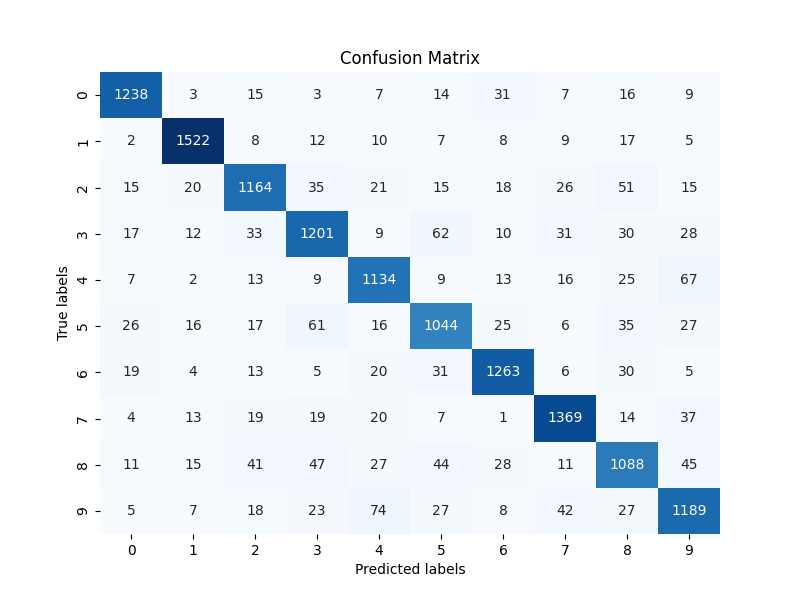
\includegraphics[width=0.8\textwidth]{images/dtcConMat.png}
    \caption{Confusion Matrix : Decision Tree}
    \label{fig:1}
\end{figure}

Best Performance by GridSearch:\\
Best parameters: \{`max\_depth': 20,`min\_samples\_leaf': 4, `min\_samples\_split': 5\}\\
Accuracy: 0.876\\

\subsection{Random Forest}
Accuracy: 0.9676428571428571 \\
Precision: 0.9676483805024302 \\
Recall: 0.9676428571428571 \\
F1 Score: 0.9676255671575715 \\
% Add confusion matrix here
\begin{figure}[H]
    \centering
    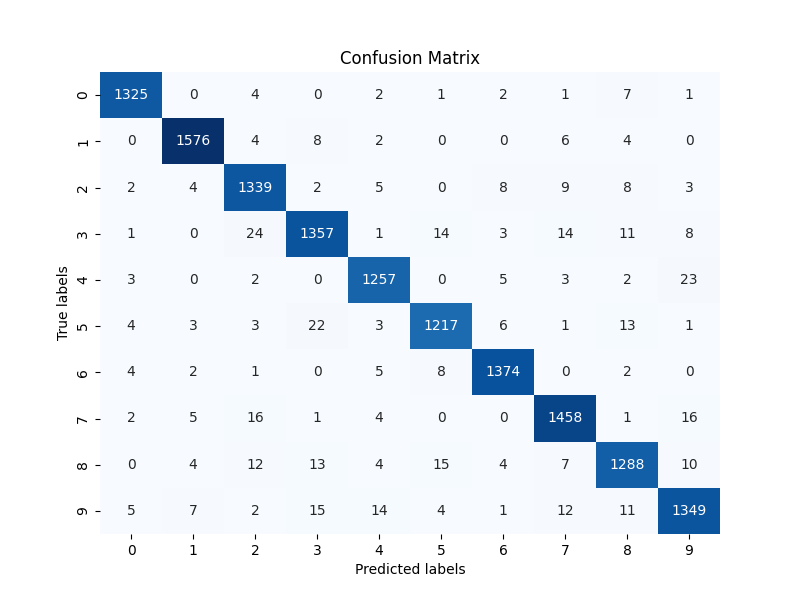
\includegraphics[width=0.8\textwidth]{images/rfcConMat.png}
    \caption{Confusion Matrix : Random Forest}
    \label{fig:2}
\end{figure}

Best Performance by GridSearch:\\
Best parameters: \{`max\_depth': None, `n\_estimators': 300\}\\
Accuracy: 0.9676428571428571\\


\subsection{Naive Bayes}
We tested three cases, and selected Bernoulli for cross-validation since it had the best performance.
\subsubsection*{GaussianNB}
0.5566 accuracy with a standard deviation of 0.0063

\subsubsection*{MultinomialNB}
0.8256 accuracy with a standard deviation of 0.0104
\clearpage
\subsubsection*{BernoulliNB}
Accuracy: 0.8348571428571429 \\
Precision: 0.8367482492867026 \\
Recall: 0.8348571428571429 \\
F1 Score: 0.8346397011541737 \\
% Add confusion matrix here
\begin{figure}[H]
    \centering
    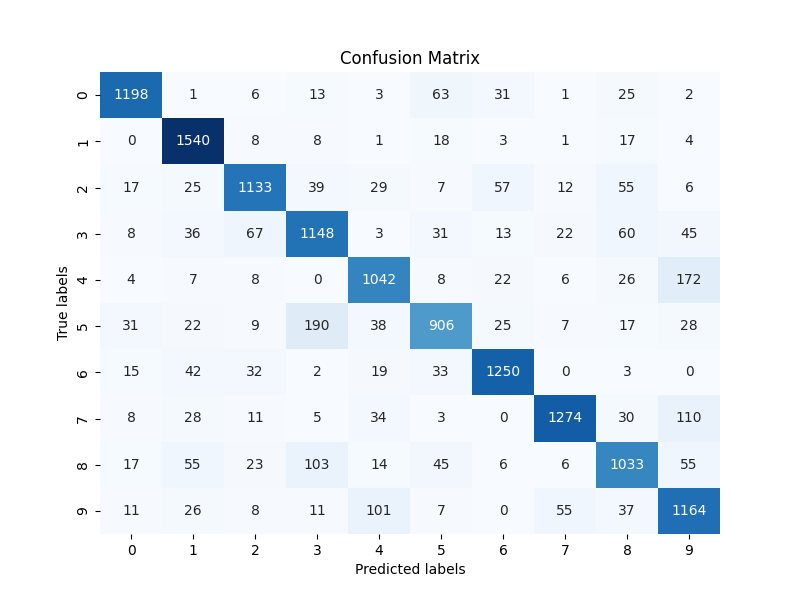
\includegraphics[width=0.8\textwidth]{images/nbbConMat.png}
    \caption{Confusion Matrix : Naive Bayes - Bernoulli}
    \label{fig:3}
\end{figure}

Best Performance by GridSearch:\\
Best parameters: \{`alpha': 0.1, `binarize': 0.0\} \\
Accuracy: 0.8352857142857143 \\
\clearpage
\subsection{KNN}
Accuracy: 0.9700714285714286 \\
Precision: 0.9702368001894589 \\
Recall: 0.9700714285714286 \\
F1 Score: 0.9700163750952855 \\
% Add confusion matrix here
\begin{figure}[H]
    \centering
    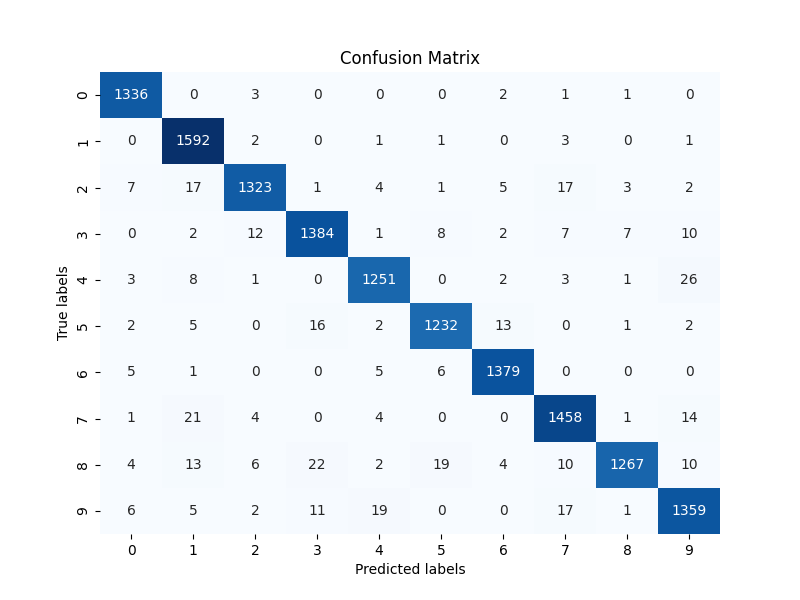
\includegraphics[width=0.8\textwidth]{images/knnConMat.png}
    \caption{Confusion Matrix : KNN}
    \label{fig:4}
\end{figure}

% Add GridSearch
Best Performance by GridSearch:\\
Best parameters: \{`n\_neighbors': 3, `p': 2, `weights': `distance'\}\\
Accuracy: 0.9728571428571429\\
\clearpage
\subsection{Neural Networks}
Accuracy: 0.9625714285714285 \\
Precision: 0.9628620900925863 \\
Recall: 0.9625714285714285 \\
F1 Score: 0.9625253215986614 \\
% Add confusion matrix here
\begin{figure}[H]
    \centering
    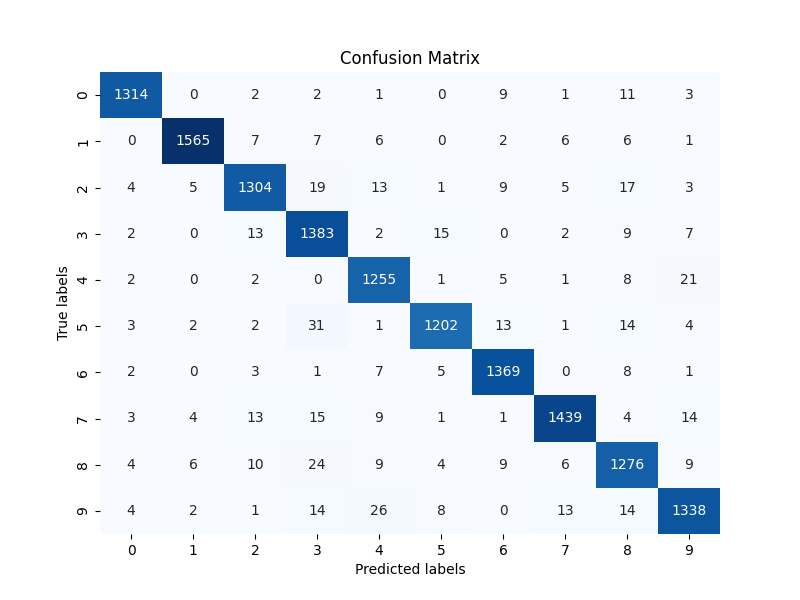
\includegraphics[width=0.8\textwidth]{images/nnConMat.png}
    \caption{Confusion Matrix : Neural Networks}
    \label{fig:1}
\end{figure}

% Add GridSearch
Best Performance by GridSearch:\\
Best parameters: \{`activation': `relu', `alpha': 0.001, `hidden\_layer\_sizes': (500,)\}\\
Accuracy: 0.9741428571428571\\

% \todo{Table}
\clearpage
\section{Grid Search Cross Validation}
\begin{table}[htbp]
    \centering
    \rowcolors{2}{lightblu}{white}
    \begin{tabular}{ll}
        \rowcolor{blue}
        \textbf{\textcolor{white}{Model}} & \textbf{\textcolor{white}{Accuracy}} \\
        Decision Tree                     & 0.876                                \\
        Random Forest                     & 0.9676                               \\
        Bernoulli NB                      & 0.8353                               \\
        KNN                               & 0.9728                               \\
        Neural Network                    & 0.9741                               \\
    \end{tabular}
    \caption{Model Comparison}
    \label{tab:model_comparison}
\end{table}

\section{Glossary}
$$\text{Accuracy} = \frac{TP+TN}{TP+FP+TN+FN}$$
$$\text{Precision} = \frac{TP}{TP+FP}$$
$$\text{Recall} = \frac{TP}{TP+FN}$$
$$\text{F1 Score} = \frac{Precision\times Recall}{Precision+Recall}$$

%\par \finalresult{Therefore, cats are equal to infinity.}
\end{document}
